\section{General Linear Model} \label{back:sec:glm}

In order to determine if a task or stimuli has made a significant contribution to the measured BOLD signal, each voxel in the scan needs to be evaluated. The following section will therefore seek to explain a method of how to determine if any significant change is found. In this project the general linear model (GLM) will be explained and applied as it is the most used and recognized tool for fMRI analysis during the past 20 years \cite{Poline2012}. 

The GLM is a well considered and used analysis tool constituting a simple way of doing standard statistical analysis on fMRI. The overall goal of the GLM model is to determine how well the time course of the scan corresponds to the known used experimental interference.  In an fMRI case that means, how well the BOLD signal over time fits the time course of the predicted signal given by the imposed stimuli, causing brain activity. This statistical test is carried out for each voxel independently of its neighbor across the scan resulting in thousands of statistical test in one scan. \cite{Moayedi2018,Monti2011} To explain the implementation of a GLM we can use the example presented by \textit{Monti et al.} An acquired BOLD signal will throughout a time series, of \textit{n} images, have a varying output signal. The signal in a voxel $Y$, at any time point, can be seen as a summation of predictor variables (stimuli regressors) $X$,  additional nuisance regressors modeling noise $X$, a scaling parameter for each regressor $\beta$, and an error term $\epsilon$. This can be presented in the GLM's basic from as \cite{Monti2011}: 
\begin{equation}
Y=X\beta+\epsilon
\end{equation}

Expanding this formulation into a complete scan, including multiple regressors, can be presented on a matrix form. A depiction of a GLM design matrix incorporating the factors making up the BOLD signal can be seen in \figref{fig:GLM}. 

\begin{figure}[H] 
	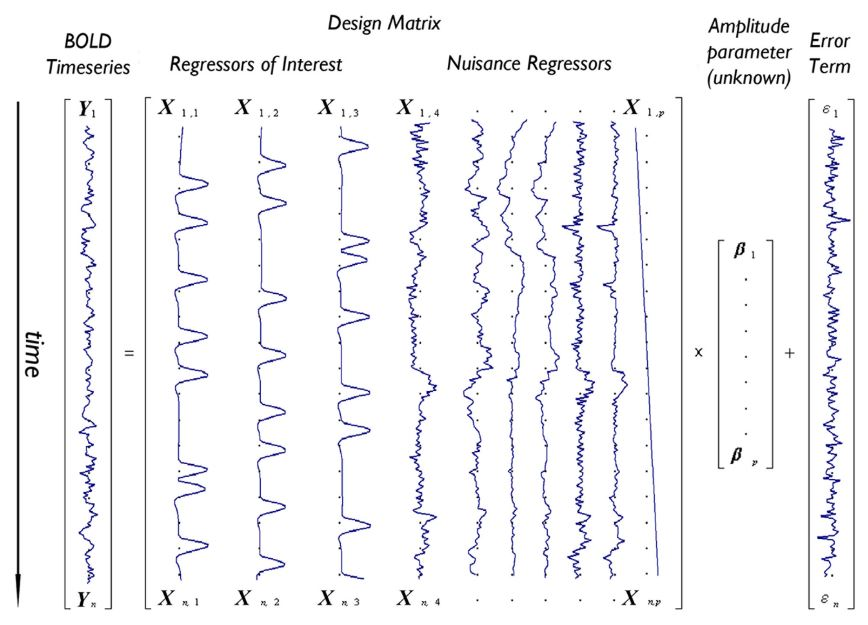
\includegraphics[width=0.90\textwidth]{figures/aBackground/GLM}
	\caption{Illustration of a design matrix for a given GLM model, describing the BOLD time series $Y_n$, the regressors of interest $X_{1,1}, X_{1,2}, X_{1,3}$, the additional nuisance regressors $X_{4..p}$, the amplitude parameter $\beta_{1..p}$ and the error terms $\epsilon_{1..n}$. \cite{Monti2011}}
	\label{fig:GLM}
\end{figure}



The predictor variables are found by modeling what is known or predicted as output. The predictors of interest would come from hemodynamic response curve convoluted with stimuli design as presented in \secref{sec:Stim}. GLM models will often introduce nuisance predictors as well used to model variables such low frequency drift and motion to make a more robust model. These are non interest regressors, as they do not resemble the wanted signal, being the stimuli induced. The amplitude parameter is the unknown weight scaling the magnitude between each predictor value and the data. They describe the strength of the relationship between that regressor and the voxel's BOLD signal course of activation. The error term contains the value for each observation, which can not be explained by the wighted sum of the amplitude parameter. \cite{Moayedi2018,Monti2011} 

The goal is to estimate the value of the scaling parameter $\beta$ for all regressors and afterwards determine if any regressor significantly account for the variance found in the BOLD signal. A regressor associated with the measured BOLD signal should hypothetically show a greater value for the voxels in the brain area corresponding to a given task. E.g. finger tapping would show greater $\beta$ values in the motor cortex. A method for estimating $\beta$ values for the regressors is the ordinary least squares (OLS). The OLS method estimates $\beta$ by minimizing the sum of squared residuals \cite{Monti2011}: 

\begin{equation}
\sum_{i=1}^{n}(Y_i-X_i\times\hat{\beta})^2
\end{equation}  

, where Y is the observed signal, X is the predicted signal which is scaled by $\beta$. $\beta$ and the variance of $\beta$ can be estimated by: 

\begin{equation}
\hat{\beta}=(X^TX)^{-1}X^TY
\end{equation}

\begin{equation}
var(\hat{\beta})=\sigma^2(X^TX)^{-1}
\end{equation}

The application of this method rest on the following assumptions being fulfilled: Error terms are independently and Gaussian distributed with zero mean, the regressors in the matrix are independent of error and non stochastic and known and no regressor is a linear transformation of another regressor. \cite{Monti2011}    




